\chapter{Modelling the thermal conductivity of Fe-bearing bridgmanite at the CMB} % Main chapter title
%(Mg,Fe)SiO$_3$

\label{Chapter4} % Change X to a consecutive number; for referencing this chapter elsewhere, use \ref{ChapterX}

As stated earlier (REF), there are no are experiments that can reach the high pressures and temperatures necessary to replicate the conditions of the lower mantle. The addition of impurities into minerals further complicates the matter. In addition to pressure and temperature-dependence, composition must be considered for full evaluation.

DISCUSS/RE-ITERATE EARLIER-DISCUSSED SEMI-RELEVANT EXPERIMENTS HERE, MANTHILAKE

%-----------------------------------------------------------
\section{Simulating the effect of atomic impurities}
%-----------------------------------------------------------

The bulk of the lower mantle comprises bridgmanite (X\%, and its high-pressure polymorph post-perovskite), ferropericlase (Y\%), along with others (Z\%) such as calcium silicate perovskite CaSiO$_3$. The composition can vary within these mineral archetypes, significantly the concentration of iron impurities. Magnesium is replaced with iron in 
\mgsios and MgO compositions, leading to \fesios and FeO endmembers. Aluminium can similarly be subsituted for Magnesium (((REF))) (Mg$^{2+}$ + Si$^{4+}$ = Al$^{3+}$ + Al$^{3+}$ or Al$^{3+}$ + Fe$^{3+}$).
BRODHOLT NATURE PAPER

Impurities reduce \tcs by providing more opportunities for phonon scattering events. An impurity is an irregularity to a propagating phonon, much like a speedbumb to a car. They have different properties to the atoms the phonon expects to meet from crystal regularity, namely mass and their bonds with neighbouring atoms. For this reason that the \tcs of a solid solution is lower at intermediate compositions than at the endmembers. Even if one endmember has lower \cs than the other, an irregular mix of the two can produce even lower values.



%---------------------------------------
\subsection{How do impurities affect conductivity?} 
%---------------------------------------
\label{impur_theory}

The effect of impurities on lattice thermal conductivity is approximated by \citet{Klemens1960} and \citet{Padture1997}, a review of which can be found in the Supplementary Material of \citet{Stackhouse2015}. The lattice thermal conductivity of a binary solid solution is given \citep[in][Eq. S6]{Stackhouse2015} as

\begin{equation}
k_{\mathrm{S}}=k_{\mathrm{V}}\left ( \frac{\omega_{\mathrm{S}}}{\omega_{\mathrm{D}}} \right )\arctan \left ( \frac{\omega_{\mathrm{D}}}{\omega_{\mathrm{S}}} \right ),
\label{SS2015SM.6}
\end{equation}
\\
where $\omega_{\mathrm{S}}$ is the phonon frequency at which the mean free path is equal to that of the solute Fe atoms, and $\omega_{\mathrm{D}}$ is the phonon frequency corresponding to the maximum of the acoustic branch in the phonon spectrum (the Debye frequency). $k_{\mathrm{V}}$ is the compositionally-weighted average of endmember conductivities, 

\begin{equation}
k_{\mathrm{V}}=\left ( 1-x \right )k_{1} + x\ k_{2} \ ,
\label{SS2015SM.7}
\end{equation}
\\
where $k_{\mathrm{1}}$ and $k_{\mathrm{2}}$ are the pure endmember conductivities, and $x$ is the decimal concentration of the second endmember \citep[][Eq. S7]{Stackhouse2015}.

Considering Eq. \ref{SS2015SM.6}, when $\omega_{\mathrm{S}} \gg \omega_{\mathrm{D}}$, $\arctan(\omega_{\mathrm{D}}/\omega_{\mathrm{S}}) \rightarrow (\omega_{\mathrm{D}}/\omega_{\mathrm{S}})$, so $k_{S} \rightarrow k_{V}$, the conductivity considering impurities tends toward the endmember linear average. This will happen when other factors, such as high temperatures, have reduced conductivity and adding impurities has little additional effect.

On the other hand, when $\omega_{\mathrm{D}}\gg\omega_{\mathrm{S}}$, $\arctan(\omega_{\mathrm{D}}/\omega_{\mathrm{S}})\rightarrow\pi/2$, but $(\omega_{\mathrm{S}}/\omega_{\mathrm{D}})\ll\pi/2$, so $k_{\mathrm{S}} < k_{\mathrm{V}}$, and impurity scattering has an effect on the resultant conductivity. Adding impurities has an effect like this when the conductivity has not already been reduced for other reasons, like at low temperatures compared to the conditions mentioned above. 

That factors which affect the severity of impurity scattering are temperature, the mass difference between the impurity and what it replaced, and the concentration of said replacements. The ratio of the phonon frequencies in Eq. \ref{SS2015SM.6} can be expressed \citep[][Eq. S11]{Stackhouse2015} as

\begin{equation}
\left ( \frac{\omega_{S}}{\omega_{D}} \right )^{2} = \frac{1}{\left ( 6\pi^{2} \right )^{1/3}} \ \frac{T}{3 \varepsilon T_{S}} \ ,
\label{SS2015SM.11}
\end{equation}
\\
where $T$ is temperature, $T_{\mathrm{S}}$ is the temperature at which the phonon mean free path length approaches that of the interatomic seperation, and $\varepsilon$ is related to the mass difference and proportion of endmembers by

\begin{equation}
\varepsilon = \frac{\left (M_{2}-M_{1}  \right )^{2}}{\overline{M}^{2}} \ x\left ( 1-x \right ) \ ,
\label{SS2015SM.9}
\end{equation}
\\
where $M_{i}$ is the atomic mass of the $i$-th endmember, $\overline{M}$ is the mean atomic mass of the solid solution, and $x$ is the proporition of endmembers \citep[][Eq. S9]{Stackhouse2015}.

As the temperature increases, so too does the left-hand side of Equation \ref{SS2015SM.11}. As discussed above, this reduces the effect of scattering caused by impurities, which will be relevant at CMB conditions. 

$\varepsilon$ increases with the mass difference of the endmembers, and the impurity concentration. Increasing $\varepsilon$ tends to reduce the phonon frequency ratio, meaning impurity scattering will affect the resultant conductivity more. The atomic masses of Mg and Fe are 24 and 56, so \fesios is 1.32 times heavier than \mgsio. As an aside, Equation~\ref{SS2015SM.9} predicts that isotopic variations will have little effect on conductivity, where the mass changes are typically small (e.g. $^{24}$Mg to $^{25/26}$Mg) and abundances are low (Mg standard atomic weight is 24.3, the ratio of $^{24}$Mg to heavier isotopes is roughly 4:1).

The composition control term in Equation~\ref{SS2015SM.9}, $x(1-x)$, increases from 0 to 0.25, when $x = 0.5$. $\varepsilon$ increases with composition up to 50\%, the furthest point away from both endmembers, therefore the condition of most disorder in the atomic structure.

!!! 181012 TALK ABOUT THESE EFFECTS AT CMB SPECIFICALLY and how they relate to the questions i'm posing?



%-----------------------------------------------------------
\section{Methodology}
%-----------------------------------------------------------

In this section I outline the process of taking Fe from chemistry to computer, by fitting my own coefficients to a Buckingham potential. I also go over how the Fe is incorporated into the \mgsio, considering its placement and concentration.

%---------------------------------------
\subsection{How does iron behave?} 
%---------------------------------------

I use two methods to introduce iron impurities to my bridgmanite models. The first approach is to simply create a magnesium atom with the mass of an iron atom, without changing any coefficients of the interatomic potentials from \citet{Oganov2000}. Despite being an obviously "quick and dirty" method, (I will show) this is a reasonable first-order approximation(((PROVE IT!?))). As the variation in mass number from Mg to Fe is large (24 to 56, a 133\% increase), it is likely to change the behaviour of the system more than a subtle change in the atomic interactions.

MENTION AMMANN IRON STUFF HERE

The second approach to add Fe into the \mgsios system is to fit interatomic potentials, as well as using the aforementioned mass change for a more realistic model. I adapted the \citet{Oganov2000} \mgsios Buckingham interatomic potential ($U$) to include the Fe-O interation. I determined two short-range potential parameters, $b$ and $\rho$, shown in Eq. 11 from \citet{Oganov2000},

\begin{equation}
U_{ij}\left ( R_{ij} \right ) = \frac{z_{i}z_{j}}{R_{ij}} + b_{ij}\ \textup{exp}\left ( - \frac{R_{ij}}{\rho_{ij}} \right ) - \frac{c_{ij}}{{R_{ij}}^{6}}, \label{og_buck}
\end{equation}
\\
where $ij$ refers to an atom pair, $R$ is interatomic distance, $z$ is atomic charge, and $c$ relates to the Van der Waals force (zero for non O-O interactions). We determine $\rho$ in the same fashion as \citet{Oganov2000}, calculated from the atomic first ionisation potentials,\\
\begin{equation}
\rho_{ij} = \frac{1.85}{\sqrt{I_{i}}+\sqrt{I_{j}}}.  \label{urusov}
\end{equation}
\\
$b$ is constrained using the GULP code \citep{Gale1997}, using the calculated $\rho$ value for Fe-O. We fit to the elasticity results of \citet{Parise1990}, an experimental study of (Mg$_{0.9}$,Fe$_{0.1}$)SiO$_3$ bridgmanite up to 433~K. Despite potential fitting being an improvement on solely changing mass (((PROVE IT!?))), it is still not perfect as the charge of our fitted Fe is not varied from the original Mg.

!!! Validate potentials
!!! Validate Fe vs. heavy Magnesium
!!! Include Oganav table (earlier?), with the fitted Fe info


%---------------------------------------
\subsection{Where do the impurities go?} 
%---------------------------------------

Iron is substituted with magnesium into the bridgmanite atomic structure. The unit cell contains 4~Mg atoms, and the smallest direct method cell I employ is a 6x2x2 supercell. Therefore the smallest amount of iron that can be added is 1/96 atoms, a concentration just over 1\%. A simple script (((INCLUDE IN APPENDIX, MENTION MATLAB?))) is used to modify LAMMPS input files, randomly selecting a specified proportion of Mg atoms to be replaced with Fe. When a Mg atom changes to Fe, its mass and interatomic potential properties change. 

Due to the microscopic nature of the system, we do not want all of the added iron to be concentrated together in the simulation cell, especially in a heat source/sink region (((ELABORATE WITH FIGURE?))). To avoid this we order Mg atoms by length along supercell, and change a single atom every so many. For example, changing 1/4 atoms is different to changing 24/96. The latter has a higher variance in Fe per unit length, and the former chooses one atom to swap for every four along the system. After iron is added, the standard direct method or Green-Kubo workflow is followed.

!!! NICE PICTURE/DIAGRAM HERE?
!!! Comparison of random and homogeneous distribution




%-----------------------------------------------------------
\section{Results}
%-----------------------------------------------------------

% reference SS2015 supp. for this section, the what affects conductivity bit
% have I gone too far into discussion here, interpretation of results?
Lattice thermal conductivities obtained from Green-Kubo calculations are plotted against temperature in Figure \ref{fig:kappa-temp_01}, for Mg and Fe-endmembers and the 50/50 solid solution mix.

Conductivity decreases with temperature, approximately following $\kappa \propto 1/T^{0.9}$ at the studied 136~GPa. This is in contrast to the typically expected $\kappa \propto 1/T$ relation, indicating some kind of saturation in conductivity decrease with temperature.

\fesios has a consistently lower conductivity than \mgsio, which is to be expected due to the atomic mass increase [WRONG, SHEAR MOD DECREASE, DENSITY INCREASE, WAVESPEED EQUATION]. The two trends appear to be converging, indicating the conductivity of both species may be equal given a high enough (though unphysical for the lower mantle) temperature. This suggests there is a minimum conductivity associated with the crystal structure, reached first by \fesios with its inherently lower conductivity.

The 50\% solid solution has a consistently lower conductivity than \mgsio, and a lower than or equal to relation to \fesios. This is again to be expected, conductivity decreases from endmember to intermediate compositions as inpurity concentration increases. It can be seen that conductivity differences are very small at high temperatures for \fesios and the solid solution. If \fesios has already reached its theoretical minimum, adding impurities will do little to decrease it further.

\begin{figure}[h!]
  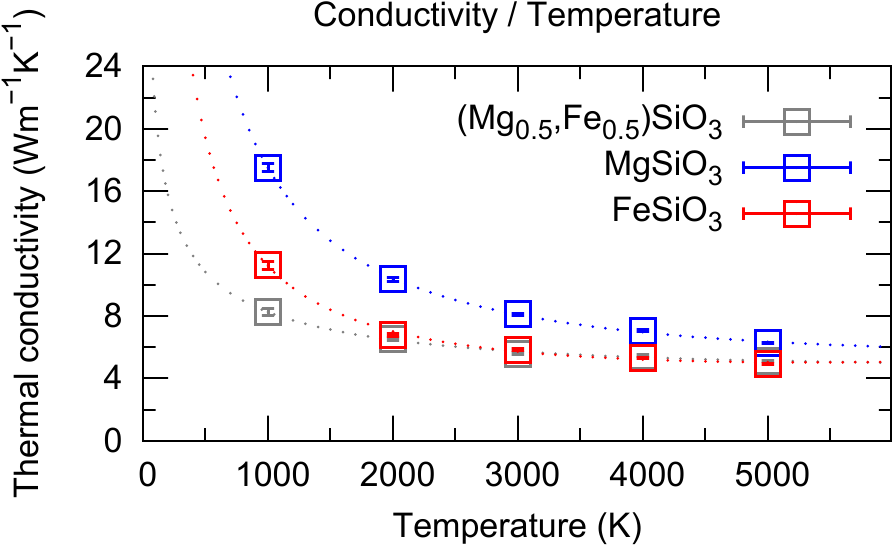
\includegraphics[width=\linewidth]{Figures/k-t_all_02.png}
  \caption{Data points are GK conductivity results, dotted line is the fit from Equation \ref{eq.okuda5_mod}.}
  \label{fig:kappa-temp_01}
\end{figure}

An alternative perspective to Figure \ref{fig:kappa-temp_01} is presented in Figure \ref{fig:kappa-comp_01}, where Green-Kubo conductivity results are plotted as a function of Fe impurity content for several temperature series.

Conductivity generally decreases with increasing temperature at all compositions, though the change becomes minimal at tempertatures above 3000~K.

The \mgsios endmember has a consistently higher conductivity than the \fesio. This can be explained by the general reduction in shear modulus and increase in density associated with adding Fe, which decreases seismic velocity and thus conductivity [TRUTH ALERT, REF???].

The amount of Mg atoms replaced with Fe has a variable effect on conductivity. A better way to label the effect is impurities added to an endmember, i.e. Fe is added to \mgsios and Mg to \fesio, which always serves increase phonon scattering and decrease conductivity. The decrease from this effect saturates towards a 50\% compositional mix. At high temperatures, this effect is minimal when adding Mg to \fesio. The conductivity could already be close to its theoretical minimum due to temperature effects, little reduction is observed from adding impurities.

\begin{figure}[h!]
  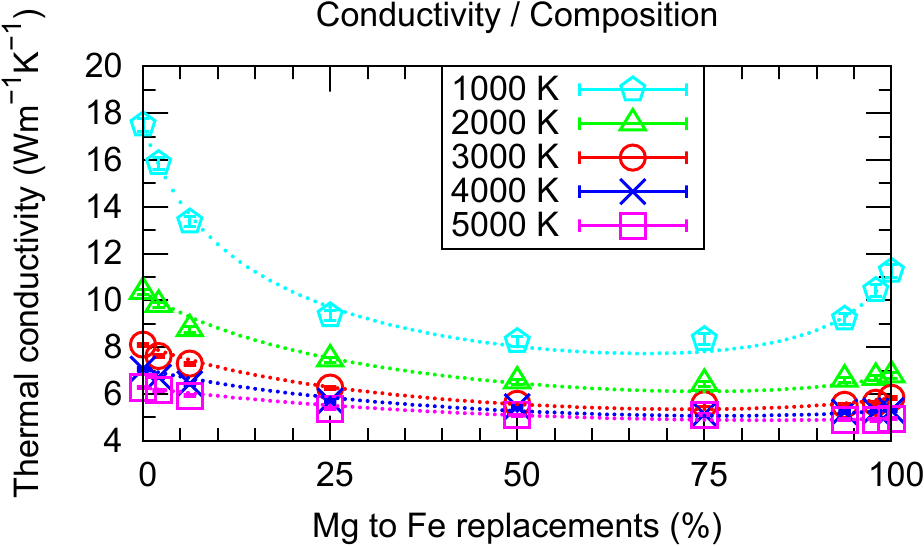
\includegraphics[width=\linewidth]{Figures/k-c_all_01.png}
  \caption{CAPTION}
  \label{fig:kappa-comp_01}
\end{figure}

A simple interpolation between endmember conductivities is insufficient, the presence of a compositional mix has an effect. This effect is itself temperature-dependent, the trough-like trend flattens with increasing temperature. These temperature and compositional dependences can be combined, allowing conductivity to be determined for a range of possible CMB conditions (Figure \ref{fig:kappa-temp-comp_01}). 

\begin{figure}[h!]
  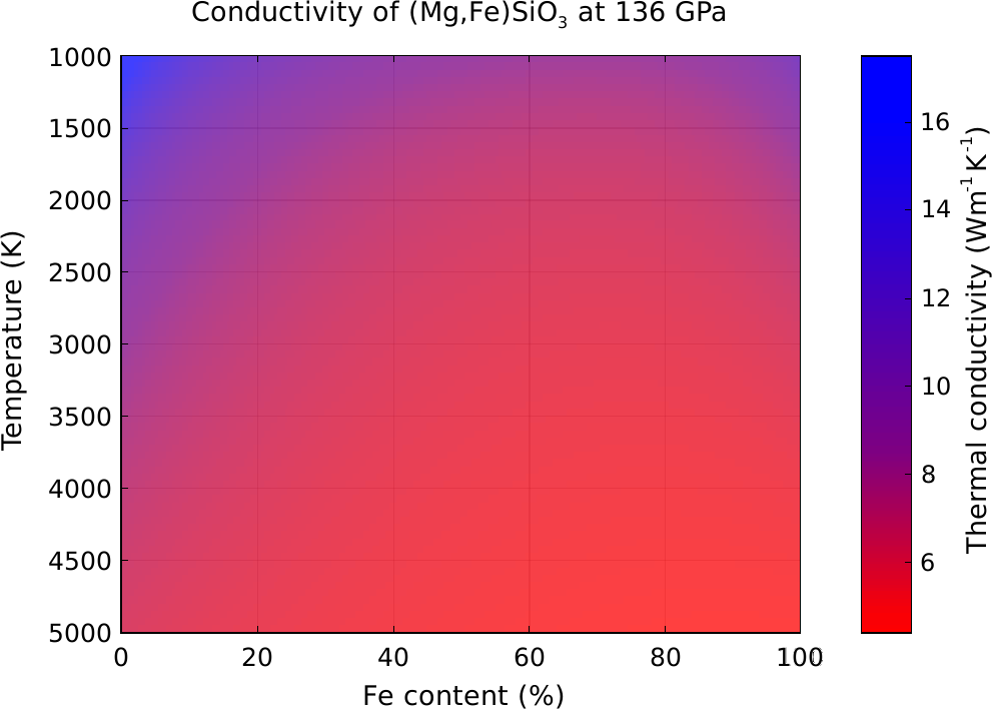
\includegraphics[width=\linewidth]{Figures/K_over_T_over_X.png}
  \caption{Modelled conductivity, shown plotted against temperature and composition. Note the sensitivity of the colour scale, showing low conductivities as dominant at high temperatures and intermediate compositions. High values are found only at low temperatures, and even then they rapidly decay and saturate to <8\wmk. Such conditions are unphysical at 136~GPa within the lower mantle.}
  \label{fig:kappa-temp-comp_01}
\end{figure}



%-----------------------------------------------------------
\section{Making the mantle model}
%-----------------------------------------------------------

I want to determine a model for the lattice thermal conductivity of \mgfesios perovskite at CMB conditions. Whilst the CMB is a small section of the lower mantle, it marks the heat flow boundary from core to mantle, making it a very interesting region for studies of on both sides of the interface. The pressure is always 136~GPa, but I am interested in how temperature and Fe-content affect bridgmanite \tc.

Due to uncertainty in the lower mantle's compositional distrubution, properties like \tcs are averaged considering the abundance of each mineral component. There are also mineral solid solutions to consider however, particularly the concentration of Fe impurities in \mgsios towards \fesio, and the phase boundary between bridgmanite and \mgsios post-perovskite. 

The conductivity of an intermediate member in a solid solution is not a simple weighted average between endmembers, you cannot interpolate linearly. This can be seen in Figure \ref{fig:kappa-temp_01}, where the (Mg$_{0.5}$,Fe$_{0.5}$)SiO$_3$ results do not plot between those of \mgsios and \fesio.



%%%%%%%%%%%%%%%%%%%%%%%%%%%%%%

%---------------------------------------
\subsection{Parameterising the data fit} 
%---------------------------------------

[Equations from \cite{Ohta2017} (eq. 7,8,9), and \cite{Okuda2017} (eq. 5)]

Equations and functional forms exist to determine the temperature and compostional dependence of \tc, and it is possible to combine the two. The basic idea is to determine the conductivity of \mgsios and \fesios endmembers at the temperature of interest, and then apply the (temperature-dependent) effect of composition.

\citet{Padture1997} propose a model for how impurities affect lattice thermal conductivity of a solid soultion, which \citet{Ohta2017} apply to experimental ferropericlase data. Following a similar methodology, I will be fitting constants that apply this compositional dependence to (Mg,Fe)SiO$_3$ perovskite results at various temperatures (1000~K, 2000~K, 3000~K, 4000~K, and 5000~K). In an additional step, I establish the temperature-dependence of the fit constants. This means I am able to quantify the effect of composition at all temperatures.

\citet{Okuda2017} present a temperature scaling relation for lattice conductivity \citep[originally from][]{Manthilake2011}, fit to their experimental results of bridgmanite. I apply this temperature scaling to computational results of \mgsios and \fesios at 136~GPa. With the temperature dependence of these endmembers and of the compositional effect, I am able to able to determine the conductivity of any composition, at any temperature in the range 1000~K to 5000~K, at 136~GPa representative of the CMB.

The aforementioned temperaturedependence from \citet{Manthilake2011} considers density, allowing conductivity to be determined as a function of temperature and pressure. In the examples I will present, I am only concerned with systems at 136~GPa. All density changes will result from thermal expansion, and the equations will be altered to accomodate this.

Some of the equations in the following section have already been presented as analogous forms in Section \ref{impur_theory}. The equations are kept similar to their published form, which was \citet{Stackhouse2015} in the former, and \citet{Ohta2017, Okuda2017} in the following.


    
%-------------------
\subsubsection{Compositional dependence}
%-------------------

\citet{Ohta2017} Eq.~7
\begin{equation}%-----
\kappa_{latt}=\kappa_{i}\left ( \frac{\omega_{0}}{\omega_{M}} \right )\mathrm{arctan}\left ( \frac{\omega_{M}}{\omega_{0}} \right )
\label{eq.ohta7}
\end{equation}%-------
\\ $\kappa_{latt}$ - output conductivity as function of t \& x (\wmk), considering mineral specific parameters\\
$\kappa_{i}$ - the composition-dependent conducitivity, if it were linearly interpolated between endmembers (\wmk)\\
$\omega_{0}$ - \enquote{\textit{the phonon frequency where the intrinsic mean free path is equal to that due to solute atoms (or just interatomic spacing?)}}\\
$\omega_{M}$ - \enquote{\textit{the phonon frequency corresponding to the maximum of the acoustic branch of the phonon spectrum (Debye frequency)}}\\

The two components $\kappa_{i}$ and $\omega_{0}/\omega_{M}$, are both temperature and composition-dependent. $\kappa_{i}$ gives the compositionally-weighted average conductivity, a linear interpolation between endmembers at a certain temperature. $\omega_{0}/\omega_{M}$ controls the conductivity decrease due to the impurity effect, the magnitude of which depends on the temperature and composition of interest.

By combining models for the temperate-dependence of \mgsios and \fesio-endmember conductivities, and the fit $\chi^{T}$ parameter, I obtain a function for conductivity of the lower mantle (136~GPa) as a function of just temperature and composition (as illustrated in Figure. \ref{fig:kappa-comp_01}).\\




Ohta eq. 8 
\begin{equation}%-----
\left ( \frac{\omega_{0}}{\omega_{M}} \right )^{2}=\frac{\chi^{T}}{C\left ( 1-C \right )}  
\label{eq.ohta8}
\end{equation}%-------
$\omega_{0}$ - \enquote{\textit{the phonon frequency where the intrinsic mean free path is equal to that due to solute atoms (or just interatomic spacing?)}}\\
$\omega_{M}$ - \enquote{\textit{the phonon frequency corresponding to the maximum of the acoustic branch of the phonon spectrum (Debye frequency)}}\\
$\chi^{T}$ -temperature-dependent parameter to \dots ??? \\
$\chi$ - \enquote{\textit{a constant}}\dots\\
$T$ - temperature of interest (K, default data fit between 1000 - 5000 K, but extrapolation should be reasonable)\\                    
$C$ - composition mix of interest (dimensionless, values between 0 and 1)\\

The equation splits $\omega_{0}/\omega_{M}$ into its temperature and composition-dependent components, where $\chi$ is a temperature-dependent variable. A value for $\chi$ is fit for all compositions at each temperature. $C\left ( 1-C \right )$ is largest when $C=0.5\ or\ 50\%$, relating to the shape of the trough formed by this fit.\\

$\chi^{T}$ scaling 
\begin{equation}%-----
\chi^{T}=A T^{B}
\label{eq.chi_scale}
\end{equation}%-------
\\ *$\chi^{T}$ -temperature-dependent parameter to \dots ??? \\
*$\chi$ - \enquote{\textit{a constant}}\dots\\
*$T$ - temperature of interest (K, default data fit between 1000 - 5000 K, but extrapolation should be reasonable)\\                    
$A$ - coefficient in $\chi^{T}$ variation with temperature\\
$B$ - exponent in $\chi^{T}$ variation with temperature\\

In order to obtain an equation for conductivity at any mantle temperature, it is required that $\chi$ can be expressed as function of temperature. Figure \ref{fig:draft_xt} shows $\chi$ over $T$ fit with a power law and 4th order polynomial, the former of which is a poor fit and the latter an egregious overfitting. 

\begin{figure}[h]
  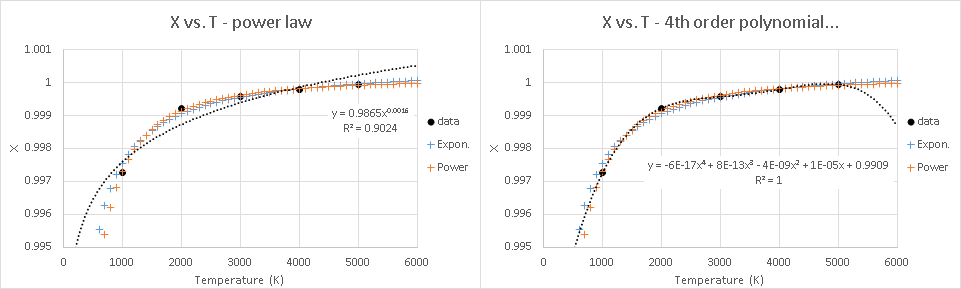
\includegraphics[width=\linewidth]{Figures/draft_XT.png}
  \caption{The fit $\chi$ values plotted against $T$, with power law (left) and 4th order polynomial (right) trendlines. Blue and orange series are the exponential and power law fits obtained from plotting $\chi^T/T$ (see Figure \ref{fig:draft_xtt}).}
  \label{fig:draft_xt}
\end{figure}

The lack of an obvious trend in $\chi$ against $T$ can be countered by plotting $\chi^T$ over $T$, and fitting either a expontial or power law relationship (Figure \ref{fig:draft_xtt}). I use the power law-relationship as it represents the temperature-dependence better, both statistically and sensitivity-wise. The value of $\chi^T$ at high $T$ has a lesser effect on the conductivity-composition relationship than at low $T$, where the power law fit matches the data closer. In Figure \ref{fig:draft_xt}, we can see that either of the power law or exponential $\chi^T/T$ fits represent the data better than the $\chi/T$ relations.\\ 

\begin{figure}[h]
  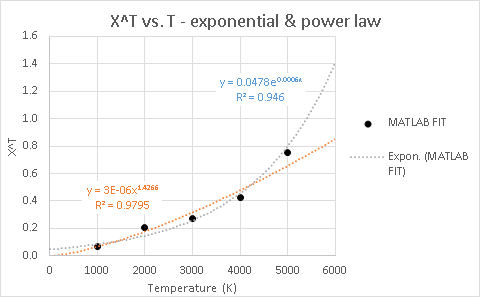
\includegraphics[width=\linewidth]{Figures/draft_XTT.png}
  \caption{Exponential fit in blue (more curved), power law in orange (flatter)}
  \label{fig:draft_xtt}
\end{figure}



Ohta eq. 9 
\begin{equation}%-----
\kappa_{i}=\left ( 1-C \right )\kappa_{\mathrm{MgSiO_{3}}}+C\ \kappa_{\mathrm{FeSiO_{3}}}
\label{eq.ohta9}
\end{equation}%-------         
\\ *$\kappa_{i}$ - the composition-dependent conducitivity, if it were linearly interpolated between endmembers (\wmk)\\
*$C$ - composition mix of interest (dimensionless, values between 0 and 1)\\
$\kappa_{MgSiO_{3}}$ - temperature and volume-dependent conductivity for Mg endmember (\wmk)\\
$\kappa_{FeSiO_{3}}$ - temperature and volume-dependent conductivity for Fe endmember (\wmk)\\

This equation describes the conductivity of an intermediate composition, assuming the relation is a simple weighted mean. $C$, in this case specifically, is the proportion of Fe atoms swapped into the system for Mg. The actual dependence of conductivity with composition is more complicated, this intermediate average value is adjusted for atomic-scale effects in Equation.~\ref{eq.ohta7} \citep[][Eq. 7]{Ohta2017}. \\

%-------------------
\subsubsection{Temperature dependence}
%-------------------

\cite{Okuda2017}\\

Okuda eq. 5 

\begin{equation}%-----
\kappa_{adj}=\kappa_{\mathrm{ref}}\left ( \frac{\rho}{\rho_{\mathrm{ref}}} \right )^{g}\left ( \frac{T_{\mathrm{ref}}}{T} \right )^{a}
\label{eq.okuda5}
\end{equation}%-------
\\ $\kappa_{adj}$ - temperature and density-dependent conductivity of an endmember (\wmk)\\
$\kappa_{ref}$ - reference conducitivty\\
$T_{ref}$ - reference temperature\\
$a$ - exponent controlling temperature-dependent conducitvity of an endmember\\
$\rho_{ref}$ - reference density\\
$g$ - exponent controlling density-dependent conducitvity of an endmember\\

\citet{Okuda2017} use a model for density and temperature-dependent conductivity (((from Manthilake 2011, REF???))), which utilises exponents obtained from REAL data / is calculated? (actually real numbers, only mine are fitted?). A reference value is scaled to infer conductivity at the conditions of interest, which in this case is temperature and pressure (via proxy using simulation cell volume/density).\\



Okuda eq. 5 modified

\begin{equation}%-----
\kappa_{\mathrm{adj}}=\kappa_{\mathrm{ref}}\left ( \frac{T_{\mathrm{ref}}}{T} \right )^{a}\left ( \frac{V_{\mathrm{ref}}}{V} \right )^{g}
\label{eq.okuda5_mod}
\end{equation}%-------
\\ $T_{\mathrm{ref}}$ - temperature at which reference conductivity is calculated (K)\\
$T$ - temperature of interest to interpolate (K, default data fit between 1000 - 5000 K, but extrapolation should be reasonable)\\   
$V_{\mathrm{ref}}$ - reference volume of an endmember (E-30 m$^3$)\\
$V$ - temperature-dependent volume of an endmember (E-30 m$^3$)\\
$h$ - exponent controlling volume-dependent conducitvity of an endmember\\

I adapt Eq. \ref{eq.okuda5} to consider volume instead of density (Eq. \ref{eq.okuda5_mod}), where density and volume are inversely proportional. Varying $a$ and $h$ I fit this equation for both Mg and Fe endmembers, using reference values from 1000~K (see Figure \ref{fig:kappa_temp_01}). The purpose of this is to scale the conductivities needed for Eq. \ref{eq.ohta9} to any temperature of interest.





\pagebreak






$$\kappa_{\mathrm{latt}}=\kappa_{\mathrm{i}}\left ( \frac{\omega_{\mathrm{0}}}{\omega_{\mathrm{M}}} \right )\mathrm{arctan}\left ( \frac{\omega_{\mathrm{M}}}{\omega_{\mathrm{0}}} \right )$$

$$\kappa_{\mathrm{i}}=\left ( 1-C \right )\kappa_{\mathrm{MgSiO_{3}}}+C\ \kappa_{\mathrm{FeSiO_{3}}}$$

$$\left ( \frac{\omega_{\mathrm{0}}}{\omega_{\mathrm{M}}} \right )^{2}=\frac{\chi^{T}}{C\left ( 1-C \right )}$$

$$\chi^{T}=A T^{B}$$

$$\kappa_{\mathrm{adj}}=\kappa_{\mathrm{ref}}\left ( \frac{\rho}{\rho_{\mathrm{ref}}} \right )^{g}\left ( \frac{T_{\mathrm{ref}}}{T} \right )^{a}$$

$$\frac{\rho }{\rho _{\mathrm{ref}}} \equiv \frac{V_{\mathrm{ref}}}{V}$$

$$\kappa_{\mathrm{adj}}=\kappa_{\mathrm{ref}}\left ( \frac{V_{\mathrm{ref}}}{V} \right )^{g}\left ( \frac{T_{\mathrm{ref}}}{T} \right )^{a}$$

$$g=\left( \partial \ln \kappa_{\mathrm{latt}} / \partial \ln \rho \right) _{T}$$

$$h \sim \left( \partial \ln \kappa_{\mathrm{latt}} / \partial \ln \rho \right) _{P}$$

$$\frac{V_{\mathrm{ref}}}{V(T)} \approx  mT+c$$

$$\kappa_{\mathrm{adj}}=\kappa_{\mathrm{ref}} \left ( mT+c \right )^{h} \left ( \frac{T_{\mathrm{ref}}}{T} \right )^{a}$$

















%Volume scaling ($y=mx+c$)  

%\begin{equation}%-----
%V=\frac{\partial V}{\partial T} T+V_{T_{0}}
%\label{eq.vol_scale}
%\end{equation}%-------     
%\\ *$V$ - temperature-dependent volume of an endmember (E-30 m$^3$)\\          
%${\partial V}/{\partial T}$ - fit gradient, change of volume with temperature (E-30 m$^3$/K)\\
%*$T$ - temperature of interest (K, default data fit between 1000 - 5000 K, but extrapolation should be reasonable)\\
%$V_{T_{0}}$ - intercept volume for T=0~K (E-30 m$^3$)\\

%I take Eq.~\ref{eq.okuda5} \citep[][Eq. 5]{Okuda2017} a step further, by obtaining $V$ in terms of $T$. This dependence is effectively linear over the temperatures considered (see Figure \ref{fig:draft_vt}). With this, Eq. \ref{eq.okuda_mod} can be made into a function of just temperature, meaning Eq.~\ref{eq.ohta7} \citep[][Eq. 7]{Ohta2017} is dependent solely on temperature, composition, and fit or calculated constants.

%\begin{figure}[h]
%  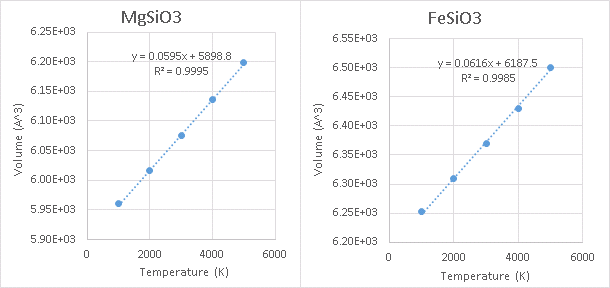
\includegraphics[width=\linewidth]{Figures/draft_VT.png}
%  \caption{Number of atoms is kept constant for all volumes, data is obtained from GK calculations of a 4x4x3 simulation cell. Magnitude of volume isn't of interest, just the relative difference to the reference volume.}
%  \label{fig:draft_vt}
%\end{figure}



\pagebreak


